\chapter[Towards a new paradigm of evaluation]{\label{chap:discussion} Towards a new paradigm of evaluation}

In the course of this thesis, we have presented several examples of an unmet assumption of the current evaluation paradigm for challenging information summarization tasks: that test collections are \textit{complete}, in that they contain the universe of all possible answers, and accurately represent the instances found in practice.
In \refchap{kbpo}, we showed how the finite incompleteness inherent in information extraction tasks, such as knowledge base population, introduces significant biases in our evaluation.
In \refchap{price}, we showed that when incompleteness is infinite, such as in text generation tasks, bias is pervasive and hard to eliminate.
Finally, in \refchap{otj}, we showed that even in complete settings such as (sequence) classification, the scarcity of annotated data makes it impossible to accurately evaluate or train systems without human intervention.
In this chapter, we will synthesize our findings on these different tasks to propose a new evaluation paradigm, on-demand evaluation, that overcomes these obstacles by asking for human feedback on system output.

More broadly, the machine learning community is trying to reconcile serious problems related to generalization even on classification tasks.
For example, even slight perturbations to the pixels of an image can wildly throw off a state-of-the-art image classification system that scores extremely well on \textit{the test set}~\citep{goodfellow2015explaining,carlini2016defensive,carlini2017adversarial}.
In fact, \citet{recht2018cifar} report a generalization gap even when the new test data is constructed in an identical (but independently collected) manner to the original training data!
Clearly, there is a problem in how we have been evaluating our systems and measuring progress thus far.
Test data that \textit{should} be representative of real-world instances does not seem to be complete.
\pl{this is mostly about train-test mis-match, which is a different problem
than the one you're addressing in this thesis;
make it clear that there are two issues}

In the field of natural language processing (NLP) field,
  there is a renewed discussion of how the performance of current NLP systems drops when applied to the real world~\citep{plank16nonstandard}:
for example, \citet{mcclosky2010any} show a 10--20 point gap between constituency parsing in domain and out of domain and \citet{foster2011news} find a similar gap on POS tagging and dependency parsing.
More recently, \citet{jia2017adversarial} find that even minor edits to the source text can throw off state of the art reading comprehension models.

Some popular routes to try and address the generalization problem include \textit{domain adaptation} (making the train and test data look more similar) and \textit{transfer learning} (measuring the speed with which a system trained on a task A can learn to perform a task B).
As \citet{plank16nonstandard} argue, domain adaptation makes the unrealistic assumption that we know what the target domain is;
  on the other hand, transfer learning may allow us to developing better learning algorithms, it does little to tell us about the performance of a system on our desired task!

Instead, we propose the new paradigm \pl{are you claiming this is novel?} of on-demand evaluation that tries to evaluate systems on real data by collecting human feedback on system output as necessary.
Much of this chapter is dedicated to synthesizing the material of this thesis to describe a more general evaluation paradigm made possible by recent advances in crowdsourcing.
Our framework tries to address the aforementioned problems with evaluation by making it more dynamic.
We close by discussing some limitations of the paradigm.

\section{The on-demand evaluation paradigm}

\begin{figure}
  \centering
  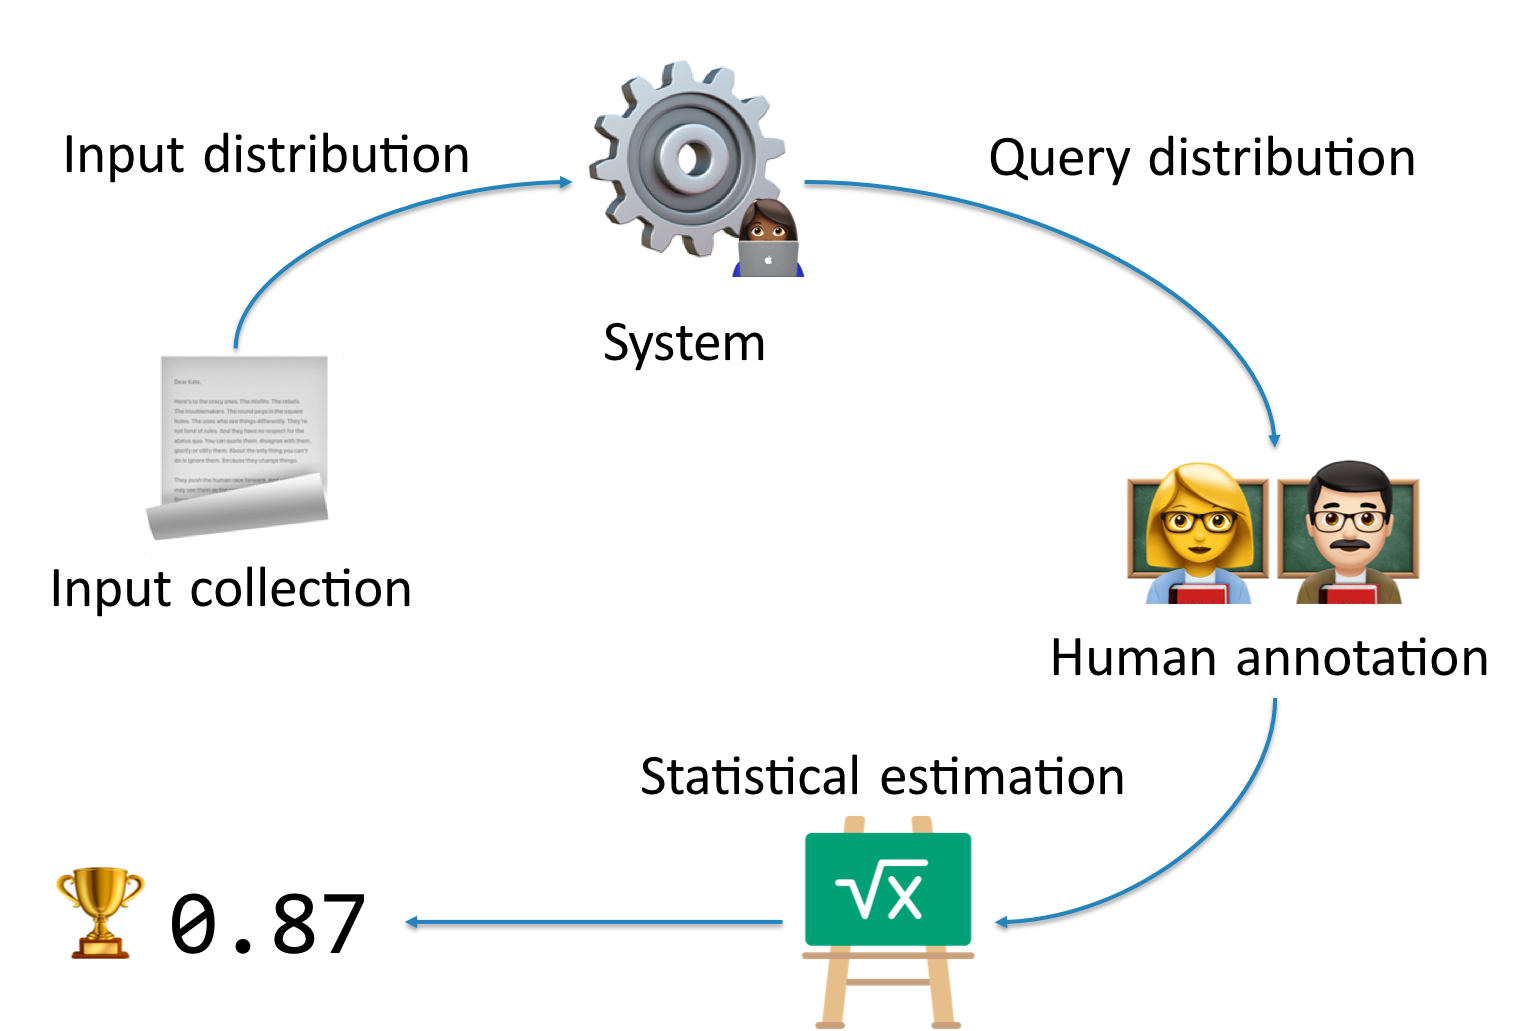
\includegraphics[width=0.9\textwidth]{figures/overview}
  \caption[Overview of the on-demand evaluation paradigm]{\label{fig:conclusions:overview}
  An overview of the on-demand evaluation paradigm. 
  First, we identify a \textit{source of inputs} (e.g.\ documents) or a distribution over the same that are provided to the system.
  Next, we specify which inputs to evaluate using a \textit{query distribution}; the query distribution plays the role of a dataset designer by identifying which system output we would like to prioritize.
  The lynchpin of the paradigm is conducting a \textit{human annotation} as necessary on the system output. 
  Finally, annotations from different systems are combined using a \textit{statistical estimator} to produce a final evaluation score.
  }
\end{figure}

\pl{I think the framing is more like: in this thesis, you've explored on demand evaluation as a way to deal with incompleteness of evaluation for hard tasks;
however, there's the general problem of evaluation, and on-demand evaluation can also be used to alleviate the issue of train-test mis-match}

The key idea of the on-demand evaluation paradigm is to bring evaluation as close to our intended use case as possible, and to overcome data incompleteness or sparsity problems by querying human annotators on-demand.
\reffig{conclusions:overview} presents an overview of the framework: 
First, the evaluation designer ensures access to a suitable stream of \textit{input examples}
which are then processed by the system being evaluated.
The evaluation designer then explicitly formulates the various goals of evaluation by specifying a \textit{distribution} over system output and input examples.
Next, the evaluation framework identifies which examples require human annotations and queries humans on-demand for these annotations. 
Finally, the annotations obtained are combined with existing annotations to evaluate the system.

We'll describe the key design decisions and challenges for each of these steps next.

\subsection{Input source}
\pl{It's not clear how general the task that this paradigm applies to is;
here we're talking about 'documents' - but those don't map to individual examples in general;
take dialogue for example
}

When identifying input examples, the evaluation designer must pick which documents to query the system on.
For example, in knowledge base population (\refchap{kbpo}), we used a large corpus of news-wire documents, which is reflective of the documents that the system would be used with in practice.
Alternatively, we could have also included a webpage crawl or documents from social media.
Another source of inputs could be actual user data (as we saw in \refchap{otj}).
Typically, the source of inputs is governed by the task.

\subsection{Query distributions}

\pl{I'm not sure in all of this what an 'example' is - input or input/output or input/prediction; make this clearer}

In the current static test-collection driven evaluation, identifying input examples is often synonymous with picking which examples to annotate and evaluate on.
\pl{isn't this the same for on-demand? you want to pick queries that represent the real world distribution}
Typically the dataset designer (e.g., the LDC in the TAC KBP tasks) identifies examples that are ``interesting'', because they provide important or challenging use cases for the system.
Often, however, there are several aspects of our systems we would like to measure at once, e.g.\ performance on particular types of entities or relations in KBP or performance on certain genres of articles in text summarization.
Each of these goals would earlier correspond to a separate set of evaluation queries. 

In the on-demand evaluation paradigm, 
  we acknowledge that it is sometimes hard to know exactly which examples should be evaluated until we obtain output from systems.
\pl{it's only the outputs that are unknown then, but the input distribution can be defined ahead of time based on what queries we're interested in, no?}
Thus, we must \textit{reify} what the goals of our evaluation are and identify specific query distributions that formalize them.
\refchap{kbpo} we saw a couple of examples of these: one query distribution could target performance of the system on particular classes, while another could focus on rare entities.
Unlike in the earlier mode of creating several separate test collections, in \refchap{kbpo} we show how we can use the same set of annotated examples to evaluate many different query distributions using importance-reweighting.

The key challenge when identifying a query distribution is ensuring that it properly reflects our evaluation goal.
Identifying the right query distribution does require some experimentation, but also allows us to draw more precise and statistically significant conclusions.
Given a static query distribution, it is usually straightforward to sample from it.
That said, it is also possible to dynamically update our query distribution during our evaluation.
In \refchap{otj} we used the system's confidence scores to dynamically decide what to annotate.
Unfortunately, an open question is what statistical guarantees we can obtain when dynamically identifying samples.

\subsection{Human annotations}
Once we have identified which examples to annotate, we must query human annotators for their feedback.
The ability to get human annotations on demand is the lynchpin of this new paradigm and is enabled by a host of modern crowdsourcing frameworks like \href{requester.mturk.com}{Amazon Mechanical Turk}, \href{https://www.figure-eight.com/}{Figure Eight} or \href{https://daemo.org}{Daemo}~\cite{gaikwad2015daemo}.
These platforms serve as labor marketplaces where it is easy and quick to hire people to answer questions, label images or text, etc.

\paragraph{Annotation interfaces.}
Having access to human annotators is particularly well suited for our purposes because the underlying difficulty when evaluating tasks such as text summarization, question answering or knowledge base population is human subjectivity.
Put differently, if our end goal is to provide summarize information \textit{for people}, it is fitting that it be judged by people as well.
At the same time, it is often non-trivial to properly communicate the subjective evaluation criteria to a non-expert annotator.
Thus, interface design and instructions are an incredibly important components when crowdsourcing.
The precise interface varies depending on the task and can range from something very simple like a Likert scale survey in \refchap{price} to something significantly more complex like the exhaustive annotation interfaces presented in \refchap{kbpo}.

Depending on the task, it may also be necessary to reformulate what annotations we obtain.
In \refchap{price}, we show that asking people to \textit{edit} a system generated summary and measuring the edit distance results in a more objective metric than simply asking for Likert scale judgments.
When annotating a linguistically nuanced task like semantic role labeling, \citet{he2015question} simplified the annotation schema by using specific questions for roles, e.g., asking ``who finished something'' in order to identify the ``agent''.

\paragraph{Interpretable annotations.}
Another consideration when deciding which annotations to solicit from crowdworkers is whether or not the annotations are \textit{interpretable}.
Interpretable annotations like the edits or highlighting justifications we collected in \refchap{price} not only make it easier to identify systematic annotation errors (which can be resolved e.g.\ by iterating on the instructions) and make the task easier to understand for the crowd worker, but also enable finer grained quantitative error analysis.
As another example, \citet{ling2017teaching} showed how natural language feedback could be used to learn how to caption images better.

\paragraph{Correcting errors in annotations.}
Despite these different approaches to improving the quality of annotations, it is hard to avoid errors made by confused or malicious workers.
Explicit models of the workers and their errors, e.g., ones proposed by \citet{dawid1979maximum}, \citet{passonneau2014benefits} or \citet{branson2017lean}, allow us to aggregate information across multiple workers to correct their errors.
In \refchap{otj}, we showed how we could use a model to dynamically identify when crowdworkers may be confused and used this information to collect additional annotations.
Such models will be necessary when evaluating complex subjective tasks like text summarization.

\subsection{Statistical estimation}
Finally, we must aggregate the human annotations to provide a meaningful quantitative score for a system.
Naively, we can always simply aggregate a suitable metric like precision, accuracy or edit distance using the human annotations, but this will not be economically scalable in the long run.
Thus, a statistical estimator that allows us to \textit{amortize} costs as we evaluate multiple systems \textit{and multiple evaluation metrics} is crucial to making the on-demand evaluation paradigm practical.
The key contribution of this thesis is showing that we can amortize costs with the appropriate statistical estimation techniques.

\paragraph{Precision and recall.}
In \refchap{kbpo}, we proposed efficient estimators for two widely used metrics, \textit{precision} and \textit{recall}.
Computing precision relies entirely on the output generated by a single system, but we showed that by using the annotations from other systems we were able to decrease the variance by a factor of four.

Accurately measuring and improving on \textit{true recall} is vital to being able to develop systems that identify \textit{new} things.
Thus far, most evaluations of open-domain tasks like knowledge base population have only reported \textit{pooled recall}, an approximation that relies on the predictions of a static collection of systems.
We showed that this approach results in a significant and systematic bias that prevents researchers from being able to measure genuine improvements.  
Instead, we leverage the recall calculated on a small, randomly selected collection of documents from the corpus.
Using our statistical estimator, we are able to correct the bias of pooled recall computed on a growing set of systems and thus decrease variance by a factor of almost four.

In both these cases, we have been able to successfully amortize costs over multiple participating systems.
The degree of cost saving really depends on the extent of overlap between systems, is best suited for problems with finite incompleteness.
We believe these techniques should easily transfer to clustering based metrics needed for entity detection and linking and co-reference resolution.

\paragraph{Black-box metrics.}
In \refchap{price}, we execute the on-demand evaluation paradigm in the setting of \textit{infinite incompleteness}, where no two systems are likely to significantly overlap in their predictions.
Of course, as a consequence, system answers also do not overlap with the reference answers in test collections.
The existing solution to this problem is to adopt a \textit{automatic metric} that serves as a similarity function between the system generated answer and reference answer.
Unfortunately, we show that existing automatic metrics not only correlate poorly with human judgment, but are \textit{biased} in that their correlations differ significantly based on the system.

In our work, we have identified an \textit{optimal} estimator to \textit{debias} these automatic metrics.
We prove that the poor correlation also fundamentally lower bounds the number of annotations need to correct the bias;
  in practice, we need almost as many human annotations to correct the bias as to conduct an complete human evaluation!
Thus, in the setting of infinite incompleteness, we have provided optimal estimation techniques, but still haven't been able to successfully amortize costs.

\paragraph{Active learning and dynamic sampling.}
Hypothetically, we could make annotation more efficient if we could dynamically pick which samples to annotate based on the systems performance on previously collected samples.
The key challenge in doing so is correcting for the sampling bias that arises as the distribution over what to sample changes every time we perform an annotation.
Unfortunately, much of the active learning literature focuses only on the generalization performance of a model trained on the samples, and not on unbiased estimation.
The dynamic annotation scheme we proposed in \refchap{otj} is able to evaluate and error-correct systems \textit{at test time}, but does not have access to a query distribution on which to compute an evaluation score.
As such, identifying an efficient, unbiased, dynamic annotation scheme is an important open problem for on-demand evaluation.

\paragraph{Quantitative error analysis.}
Apart from merely obtaining a single quantitative score with which to compare systems, the goal of evaluation is to quantify the limitations of current systems in order to provide direction for future work.
This is often manifested in authors conducting a qualitative error analysis, wherein a small sample of system output is manually inspected and coded for particular language errors.
With humans-in-the-loop, it is possible to collect far more data and conduct a more fine-grained error analysis than was previously possible.

However, by using an appropriate statistical estimator, we can also significantly decrease the costs of conduct fine-grained error analysis by efficiently reusing annotations.
As an example, in \refchap{kbpo} we show how we can accurately analyze the errors made by a knowledge base population system on different relations and entity linking without having to re-annotate any data.

\pl{I found the explanation of this paradigm a bit confusing.
The way I understand things is:
(i) you pick an input distribution (both the domain and how much you care about certain entities as in KBP, etc.); this part is static;
(ii) you collect outputs for these inputs somehow so you can at least train a system (you didn't talk about this, but I guess this is necessary?);
(iii) you run systems on all the inputs;
(iv) you adaptively figure out which input/system predictions to ask humans to annotate (is it annotation or evaluation?) and use statistics to produce meaningful numbers (unbiased, low variance, etc.);
(v) maybe use these annotations back as supervision to systems (you didn't talk about this, but would connect to online learning, which may allow you to connect on-the-job-learning ideas)
}

\pl{In general, I'm not sure I would tout this whole thing so much as a framework,
since at least right now, I don't see a single unified story that applies to all NLP tasks;
I feel like the interesting contributions are in the mechanics how to reduce variance, eliminate bias, etc.
not really in the structural aspects that a framework typically offers
}

\pl{also, you should try to really be careful about what the scope of what you're saying is:
is it AI in general (including vision tasks)? NLP tasks? relation extraction?
some of the wording really suggests something rather specific, but 'on-demand evaluation' is such a general term...
}

\section{Limitations}
Having presented an overview of the on-demand evaluation framework, let's now look at some of its limitations.

\paragraph{Cost and latency.}
While utilizing human feedback is currently necessary to evaluate the natural language processing tasks presented here,
  doing so incurs both costs to pay human annotators and latency.
In \refchap{otj}, we used ideas from game playing to strategically \textit{trade off} error rates, annotation cost and latency. 
Further improvements require new ideas.

One approach to decrease the costs of annotations is to \textit{gamify} the task to incentivize people to provide labels for their personal enjoyment.
For example, the ESP game~\citep{ahn2004labeling} was successfully able to collect thousands of image labels by asking two randomly paired people to try to label the image with the same word.
Gamification has also been applied to language tasks like word sense disambiguation~\citep{vannella2014validating} and coreference resolution~\citep{poesio2013phrase}.
For all it success, gamifying complex annotation tasks can be quite challenging, even more so if annotations are desired immediately.

The latency of acquiring human annotations can often be improved by parallelizing across multiple annotators, optimizing the annotation interface  or batching similar tasks to decrease worker context switching.
\citet{krishna2016embracing} combine all these ideas to show how images can be successfully labeled at human response times by tapping into the annotator's reflexes: once aggregated over several annotators, they are able to speed up annotation by a factor of 10 with only a small reduction in speed.

\paragraph{Integration with training.}
In this thesis, we have seen how we can properly evaluate complex natural language tasks with human feedback.
Could we use the same human-in-the-loop paradigm to \textit{train} machine-learning based systems for these tasks?
In \refchap{otj} we showed one approach that was able to use human feedback to efficiently and cost-effectively train relatively simple models.
However, many modern natural language processing systems have millions of parameters and require tens to hundreds of thousands of labeled examples:
  the cost and latency of utilizing humans-in-the-loop presents a serious bottleneck during training loop.

One approach to integrate human feedback during training is to learn how to simulate human feedback (i.e.\ learn a ``reward function'').
For example, \citet{christiano2017deep} collected human preferences on robot trajectories and found that by first learning a model of human feedback, they were able to speed up the training of the robot.
It is yet to be seen how such ideas can be extended to language tasks.
\pl{oddly specific/recent reference; this is the whole field of inverse RL; there are both classic citations and NLP-relevant ones that'd be better to add}

\paragraph{Dynamic evaluation.}
Finally, the evaluation framework we presented does not yet cover natural language tasks that need human interaction, e.g.\ dialogue systems \pl{cite dialogue evaluation paper}.
Here, the output of the system depends not only on the initial prompt, but also on every intervening response from the human and the system.
As a result, two chatbot systems answering the same initial prompt may take different trajectories based on who they are interacting with.
One of the biggest open questions is understanding what we should be evaluating in such settings and how to account for the variability introduced by the intermediate human responses.

\section{Conclusions}
In this thesis, we have introduced a new paradigm of evaluation, on-demand evaluation, that enables evaluation on complex subjective  tasks that can not be adequately captured through test collections.
We exploited advances in crowdsourcing to collect human feedback to evaluate systems as necessary and develop new statistical estimators to make efficient use of the feedback.
We have executed the on-demand evaluation paradigm on several challenging use cases, from knowledge base population to text summarization.

Still, there is much work ahead to improve the evaluation of natural language processing systems.
We hope that the discussion in this last chapter has provided some direction on where to go forward.
However, we must remain humble in recognizing the limitations of any evaluation.
As the techniques we seek to evaluate evolve, so too must our evaluation methodology.

\pl{there are some important questions/topics about evaluation that you should try to answer or at least discuss in this conclusion:
(i) what's the goal of evaluation? there's the difference between evaluation for leaderboard numbers, evaluation for providing feedback to a human (error analysis), evaluation for providing feedback to a learning algorithm (this is a big one that we've talked about a lot)?
(ii) what are the prospects for automatic evaluation (BLEU, ROUGE)? be completely practical: are you actually advising people stop doing this or is there a place for it?  what about many forms of evaluation?
(iii) do you really need evaluation to be unbiased (related to the points above)?
(iv) how does the bias problem of evalutaion relate to bias in machine learning in genreal?
(v) how important is the immediacy of getting an evaluation result?
}
